\section{COURSE INTRODUCTION}

 
VEDIC ASTROLOGY AND AYURVEDA COURSE INTRODUCTION
  Welcome to the Astrology of the Seers Course in Vedic Astrology and Ayurveda! We offer our best wishes and blessings in your studies and our connection with our teachers and traditions!  

Ours is the oldest and most widely used course on Vedic astrology, first introduced in 1985, when the subject was hardly known in the West. Many students and practitioners have learned from our course from all over the world.
Dr. David Frawley (Pandit Vamadeva Shastri), the course author, remains today probably the most widely respected western Vedic astrologer in the world, with his recognition extending throughout India by traditional astrologers there, including the highest awards by ICAS (Indian Council of Astrological Sciences) and the government of India (Padma Bhushan, the third highest civilian award for his educational work).
Our on-line course allows the student access to the course anywhere in the world and eliminates any dependency on printed course material. However, you can print the course pages as needed. For this you will need to print through your browser or cut and paste the relevant material that you wish to copy. You cannot save the course as a pdf file, download it directly or send it out as an attachment to others. This is necessary for us to protect the course material for us and its copyrights.
In addition the on-line version will allow you access to the updated course material that will be continually incorporated in the course, including new illustrations, audio and video components.
  If you ever need help with anything relative to the course, please email  us at vedicinstitute@gmail.com. Do not try to contact us by phone, though the course itself, through the website or via our social media.

\subsection{STUDY OF VEDIC ASTROLOGY}
     The field of knowledge and inner growth in Vedic astrology is unlimited, as is the degree of help and service that you can render though it. To achieve this, you should be motivated by the pursuit of truth. You are embarking on a great journey of self-discovery and are opening yourself to the whole field of Vedic, cosmic and self-knowledge. This is bound to be beneficial for you, though you should be motivated by your study, not by a seeking of results, which must come of their own accord if you are devoted in what you do.   Time, patience and steady application are the main elements that will enable your studies to become successful. You must arouse your own real interest and develop your own direct perception, adapting what you learn creatively according to your own life and temperament.  

\subsection{PURPOSE OF THE COURSE}
  The purpose of this course is twofold:

First, to provide knowledge and expertise in the basic system and fundamentals of Vedic Astrology;
Second, to introduce the student to the more specific field of Vedic medical astrology or Ayurvedic Astrology.
  This makes our course unique in that it teaches you the basic of Vedic astrology with specific reference to its Ayurvedic application. Dr. Frawley is one of the few teachers who has the highest level of recognition in both Ayurveda and in Vedic astrology.  

\subsection{BACKGROUND OF THE COURSE}
 The VEDIC ASTROLOGY AND AYURVEDA COURSE is based upon the classic book Astrology of the Seers in teaching Vedic Astrology as adapted to the global culture emerging today. The book was one of the first published in the west on Vedic astrology in 1990.   The course is based upon a thorough study of the book and uses various readings from it.  Yet the course goes far beyond the book and adds much new material. It also uses the more recent book Ayurvedic Astrology as the main text for Part II, as part of its Ayurvedic focus.  

\subsection{REQUIREMENTS OF THE STUDENT}
  The course does not presume any previous background in astrology on the part of the student, though such knowledge is helpful. Nor does it presume any astronomical knowledge on their part. The course has little mathematics or astronomy to it. I   The course does require that we have access to a computer programs and Vedic software for the more complicated calculations of Vedic Astrology, which are now easily available on the internet. Even if we can do many of the calculations ourselves, a computer program is essential because some of the more complex calculations of Vedic Astrology can take days to do manually, even by one skilled in astronomy and mathematics.   The course does require that we think, study, learn and try to apply our knowledge. Knowledge of anything, particularly such a complex subject as astrology, will not come without effort and dedication.  

\subsection{ORIENTATION OF THE COURSE}
 The purpose of the course is to bring out the universal knowledge inherent in the Vedic system, which is useful to everyone regardless of race, culture or religious background. “Veda” itself means wisdom or knowledge of truth that is based upon direct perception. It refers to univers­al knowledge, not the dogma or opinions of a particular culture. The universality of the Vedas is what is aimed at in this course – the knowledge of truth that dwells in the hearts of all. It is the knowledge of our true Self and Soul. It belongs to all of us intrinsically and is free for each of us to use regardless of our birth or backgro­und. For these reasons, we are hoping to establish a new Vedic association or Vedic Samaj to share this greater Vedic vision with all.   This course on Vedic Astrology is part of a work on various aspects of Vedic Science that the author has been engaged in for over twenty years. It includes Ayurveda, the traditional medical healing system of India, Yoga and other Vedic disciplines. Ayurveda is important in the course sections on the Astrology of Healing, which forms the basis of the second part of this course, as Ayurveda and Vedic Astrology have always been closely linked for healing purposes.   This course is based on a broader Vedic view than most presentations of Vedic Astrology. This older Vedic knowledge is specifically applied to the lunar constellations or Nakshatras, which derive directly from the Vedas. The course is also integrated into the whole system of Vedic knowledge and does not present astrology in an isolated manner.   It is in this light that we use the term “Vedic Astrology.” It has a traditional basis but cannot be fixed to a particular approach. Traditionally, Vedic Astrology has many branches and subsystems, is much more complex and allows for a greater diversity of approach than Western Astrology. Vedic knowledge itself is based upon the freedom and creative intelli­gence of the individual being. Hence, every true practitioner of it will have his or her own particul­ar version of it.    
 
 \begin{figure}[H]
 \centering
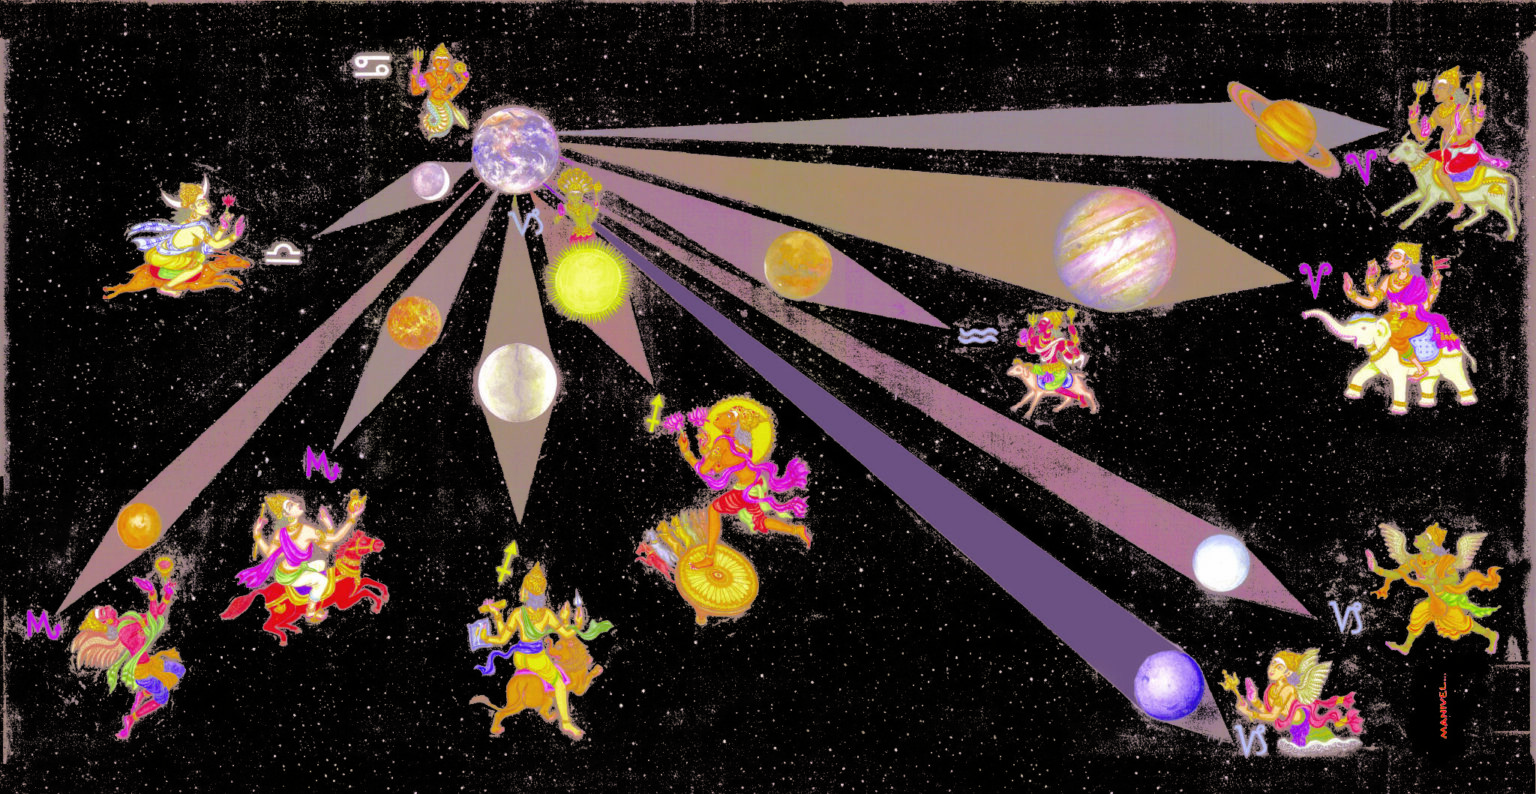
\includegraphics[width=0.8\textwidth]{pics/intro1.png}
\caption{Jyotish}
 \end{figure}

\subsection{BOOKS AND CDS FOR COURSE}
 

Astrology of the Seers: A Comprehensive Guide to Vedic/Hindu Astrology is the main book required for the course,
With Ayurvedic Astrology: Self Healing through the Stars for Part II is also required for the course.
Jyotir Bhava, Vedic astrology Mantra CD of Yogini Shambhavi Chopra (Lotus Press). This is recommended for all students wanting to know the correct pronunciation of the main mantras to the planets. Links to these chants can be found in the course and on the website.
      We generally recommend that the student complete this course material before embarking on an extensive study of traditional Hindu astrological literature, but this is left up to the discretion of the student. Traditional Hindu astrological literature can be cumbersome and without the proper background it is difficult to approach.  However, once the student has grasped the basics of the system, a study of such classics as the Brihat Parashara Hora Shastra, Brihat Samhita and Brihat Jataka (of Varaha Mihira) can be very helpful.  

\subsection{VEDIC SOFTWARE}   Many good software programs in Vedic Astrology exist notably Parashara’s Light. We recommend that the student purchase a good software programs in order to run and study charts on their own. Most software programs provide demos for you to explore and see how they work. The calculations required for Vedic charts is extremely difficult and time-consuming otherwise. There are also now some very inexpensive but more limited programs like Jyotish-D for iPhone and IPad. Note that we do not represent, nor do we receive any payment for any student who orders any Vedic software.


\begin{figure}[H]
 \centering
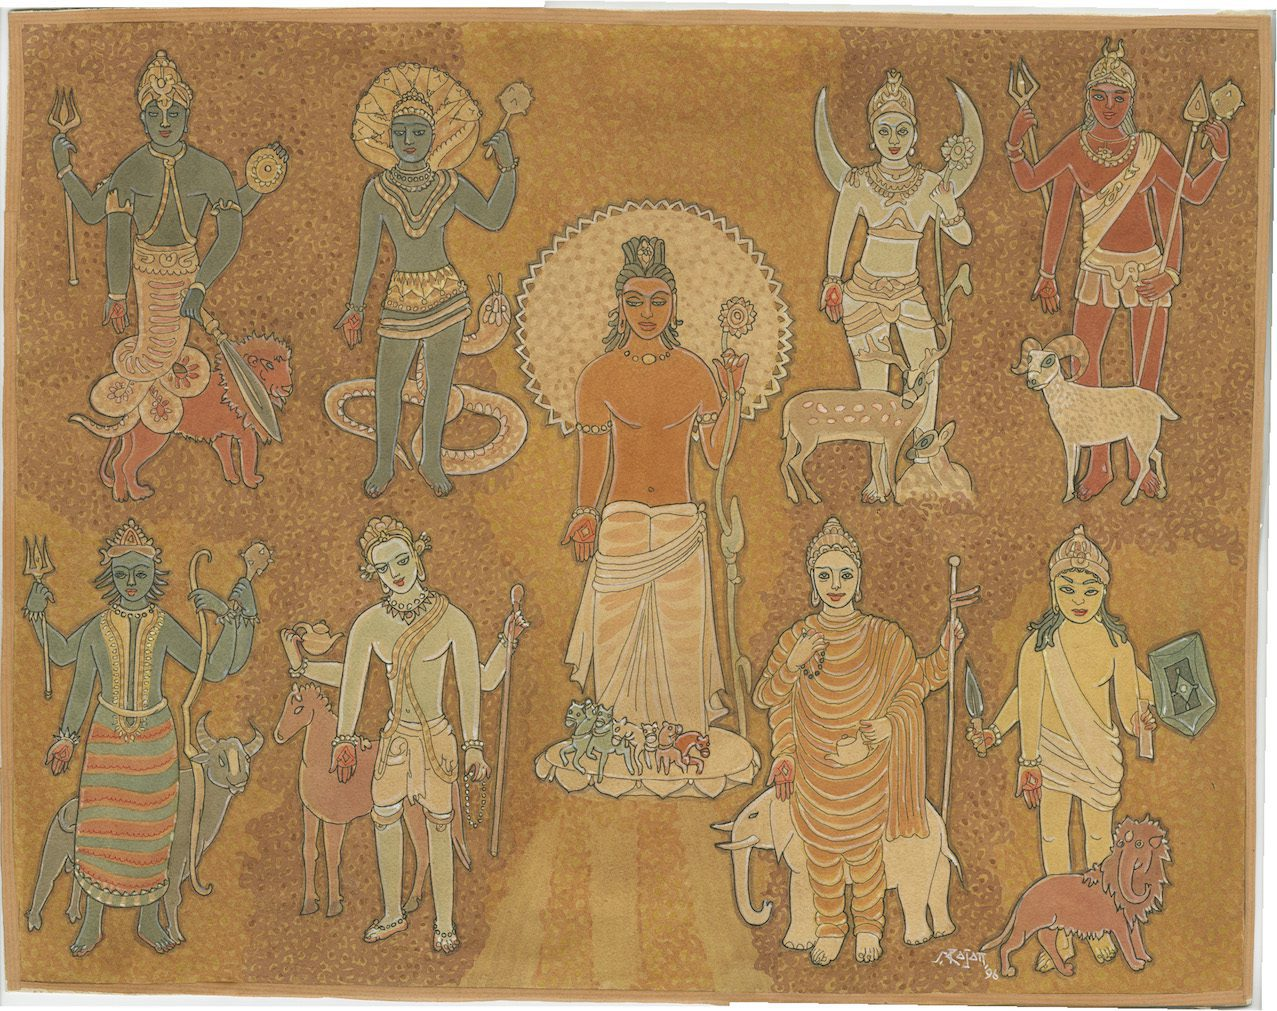
\includegraphics[width=0.8\textwidth]{pics/intro2.png}\caption{Planetary Deities}
 \end{figure}


\subsection{FORMAT OF THE COURSE}
  The course consists of 4 parts:

Part I deals with the main interpretative factors of Vedic Astrology, the foundational material.
Part II deals with Ayurveda, factors of Medical Astrology and remedial measures in Vedic Astrology.
Part III gives specialized, advanced and supplementary material on topics such as Nakshatras, Horary Astrology and Ashtakavarga.
The Workbook stands as a fourth section and is used along with the other booklets starting with Part I, will be noted in the course material.
 
\subsection{Course Workbook}
The Workbook is intended for usage in the following way:

Lessons 1-4 of the Workbook should be examined along with Part I of the course. There will be indications in Part I and at its end about this.
Lessons 5-7 of the Workbook should be examined along with Part II of the course. There will be indications in Part II and at its end about this.
You can examine the appendices in the Workbook at any time as these are for general reference.
  The Workbook is meant to provide technical and practical material, including example charts. It contains study exercises but no questions. However, a few of the questions in the tests at the end of Part I and Part II are based upon the Workbook and cannot be answered without completing it. The Workbook is particularly important for those seeking advanced training in Vedic Astrology. Others may find the Workbook to be challenging. They should be patient and realize that such application is necessary in order to learn to read charts.  

\subsection{COURSE ILLUSTRATIONS}
Course illustrations derive mainly from the Hinduism Today magazine and monastery and are under copyright. Please honor this.   COURSE AUDIOS AND VIDEOS Courses contains numerous audios and several videos to enhance the course material. These are being added to over time.  


 

\subsection{Final Test Questions}
At the end of each of the three main sections are certain Final Test Questions. The student should complete these test questions and send them to the Institute for grading.
Only if these three final tests are answered will the student receive certification for the course.
Course progression percentages are merely book marks of where in the course you have opened to the lessons. These percentages do not indicate actual course completion, which is only indicated by completion of final tests.
You can copy the tests from the on-line course material and add your answers and then send to us by email at vedicinstitute@gmail.com.
Send tests back in Word or Pages attachment. Do not send in PDF or embed in your email. This makes it easier to keep track of your tests.
Please include your name, the date you signed up for the course and your address on the test.
As it is an open book test we expect the student to answer all questions correctly.
You can also ask whatever additional questions about the course material you have along with the tests.
It usually takes us a day or two and up to a week to answer final tests. If you have not heard from us after that, please resend your tests, as sometimes tests do get lost in the spam mail.
 

\subsection{\textbf{SPECIAL AUDIO INTRODUCTION TO THE COURSE BY DR. DAVID FRAWLEY (VAMADEVA SHASTRI)}}
    

\subsection{VEDIC ASTROLOGY READINGS FOR COURSE STUDENTS}
Consultations
Those looking for Vedic astrology consultations can schedule these with Yogini Shambhavi Chopra, Shambhavi.yogini@gmail.com. Shambhavi provides an excellent approach to Vedic counseling through Vedic astrology. For students wishing to have Vedic astrological readings with us, you can arrange a reading with Yogini Shambhavi Devi (shambhavi.yogini@gmail.com), who is our resident Jyotishacharya. Yogini Shambhavi is one of the most respected women Vedic astrologers and Yoga teachers in India and the West.        Such readings can be very helpful in understanding Vedic astrology, as well as how to give readings, but are not included in the course and have their own separate charges.  

\subsection{OUR WEBSITE AND SOCIAL MEDIA}
 

Our web site at WWW.VEDANET.COM contains many articles, publications and resources.
  It includes a listing of books on Ayurveda and other Vedic topics by Dr. Frawley, and a set of over one hundred articles by Dr. Frawley on various aspects of Vedic knowledge, including sections on Ayurveda, Yoga and Vedic astrology. It contains extensive information on Yogini Shambhavi Devi, including her teachings and astrological consultations. Our various programs, intensives and travels are explained in detail. We advise the student to look at these website resources periodically for additional information in the field.  

\subsection{OUR FACEBOOK ACCOUNT FOR AMERICAN INSTITUTE OF VEDIC STUDIES} – for articles, retreats, travels and programs relative to the institute – https://www.facebook.com/americanvedic/
Dr. Frawley’s FACEBOOK ACCOUNT at https://www.facebook.com/drdavidfrawley – Regular information about Dr. Frawley and his many articles, programs and activities in the greater Vedic field, including his work in India, with over a hundred thousand followers. Not specific to Vedic astrology.
Yogini Shambhavi’s FACEBOOK ACCOUNT at https://www.facebook.com/yogini.shambhavi/ – Yogini Shambhavi’s special teachings, information and resources on Shakti Sadhana, Women’s Healing and our Yoga and Ayurveda retreats.
 Dr. Frawley’s TWITTER ACCOUNT at https://twitter.com/davidfrawleyved –  Features Dr. Frawley’s educational and social work in India, with six hundred thousand followers, which includes noted leaders, writers and spiritual teachers. Not specific to Vedic Astrology.
 

\subsection{COURSE REFUNDS AND TERM FOR COMPLETION} For such on-line courses, refund must be requested within thirty days. There will be a $50.00 processing fee taken out of the payment for our time involved. You have up to three years to access and finish the course.  

\subsection{CERTIFICATION}
  Certification for the course is given through THE AMERICAN INSTITUTE OF VEDIC STUDIES. The course provides certification for 300 hours of study in Vedic Astrology (which is how long the course, its exercises and tests, and books should take to complete), and the title AYURVEDIC ASTROLOGER: FOUNDATION COURSE.   As our institute has its own global recognition, this certification has value in its own right, particularly for combining Ayurveda with Vedic Astrology. You can also call yourself a student of Dr. Frawley, who is one of the most respected Vedic teachers in the world today.   Certification in this distance learning course does not mean that you are a fully qualified Vedic Astrologer but that you have a good foundation of information in which to become one. The course is a first stage in training in Vedic Astrology, which usually takes two years in order to become competent in the subject, like any technical discipline or profession. Yet it provides you much useful information to use for the rest of your life.  

\subsection{FURTHER TRAINING OPTIONS WITH US} Additional Programs

This course goes along with our other online courses, Ayurvedic Healing for those who wish to study Ayurveda more deeply, Integral Vedic Counseling for those interested that topic, and Yoga, Ayurveda, Mantra and Meditation for those who wish to integrate the spiritual and psychological aspects of Yoga and Ayurveda.
Dr. Frawley does take on a few students for special advanced training with him personally.
Integral Vedic Master Educator Certification, Ayurveda, Raja Yoga, Vedic Astrology, Vedic Counseling. For select students who have completed all our four courses and want a background recognition of the interconnection of their studies.
For advanced study you may consider more in-depth programs on any of the Vedic Sciences, if you have not studied these, including Yoga, Ayurveda, Vedic Astrology and Vastu. Note our courses in these fields. You might also want to take consultations with various practitioners in these fields. Dr. Frawley takes on a few private students. You can contact us if you are interested in this option. Generally this is limited to those who already have studied, practiced or taught the Vedic teachings for a number of years. It usually requires that you attend some of our retreats as well

Dr. Frawley is available for special Vedic Counseling Sessions that can also help guide you in your Vedic Counseling Practice.
 

May your study and practice of Vedic Astrology prove fruitful, transformative and enlightening! Sri Veda Purushaya Namah! Dr. David Frawley (Pandit Vamadeva Shastri)  

Namaste! 

\subsection{INDIAN NATIONAL TELEVISION (DOOR DARSHAN) INTERVIEW WITH DR. DAVID FRAWLEY}
The link is to aninterview of Dr. Frawley that explores his approach to Vedic knowledge, including Vedic astrology. For those of you who are not familiar with the scope of his work, please view it. It will help you understand the spiritual and philosophical background for this course. With Rajiv Mehrotra, not film maker and associate of the Dalai Lama. You can view it directly here. \url{https://www.youtube.com/watch?v=O0uxv-KBQgA}

